\section{Experiment design and data gathering}

In designing our experiment, the first step is to carefully select a set of excitation frequencies. 
These frequencies play a crucial role in characterizing the behavior of the system under study. 
We typically consider the following frequencies:
\begin{itemize}
    \item The Nyquist frequency, denoted as $\omega_N$.
    \item The maximum explored frequency, denoted as $\omega_H$.
\end{itemize}
It's common practice to ensure that the maximum explored frequency $\omega_H$ is significantly lower than the Nyquist frequency $\omega_N$.
\begin{figure}[H]
    \centering
    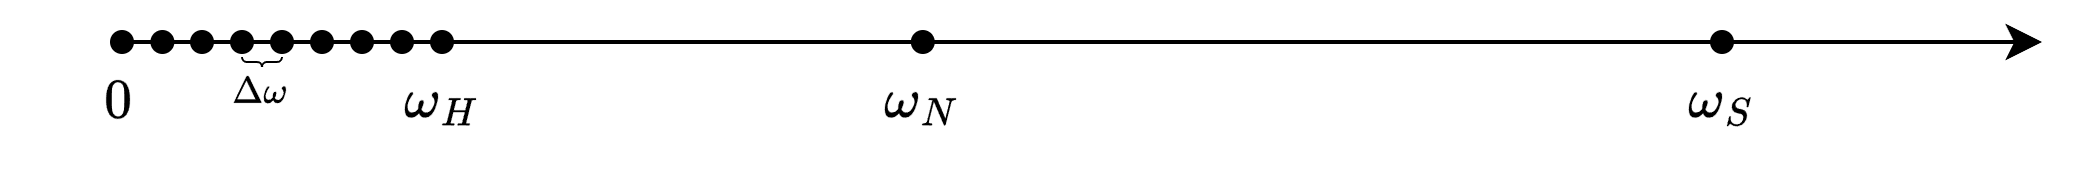
\includegraphics[width=1\linewidth]{images/experiment.png}
    \caption{Physical system}
\end{figure}
Within our experiment design, $\Delta\omega$ represents the step size between two consecutive explored frequencies. 
Typically, this step size remains constant, facilitating an even distribution of frequencies from $\omega_1$ to $\omega_H$. 
Hence, the set of explored frequencies can be represented as $\left\{\omega_1,\dots,\omega_H\right\}$. 

Our primary objective is to identify an effective model that accurately represents the behavior of the system across this range of frequencies.

\subsection{Experiments design}
To comprehensively explore the behavior of the system, we conduct $H$ independent input-output experiments. 
Each experiment involves applying a specific excitation signal to the system and observing its response. 
\begin{figure}[H]
    \centering
    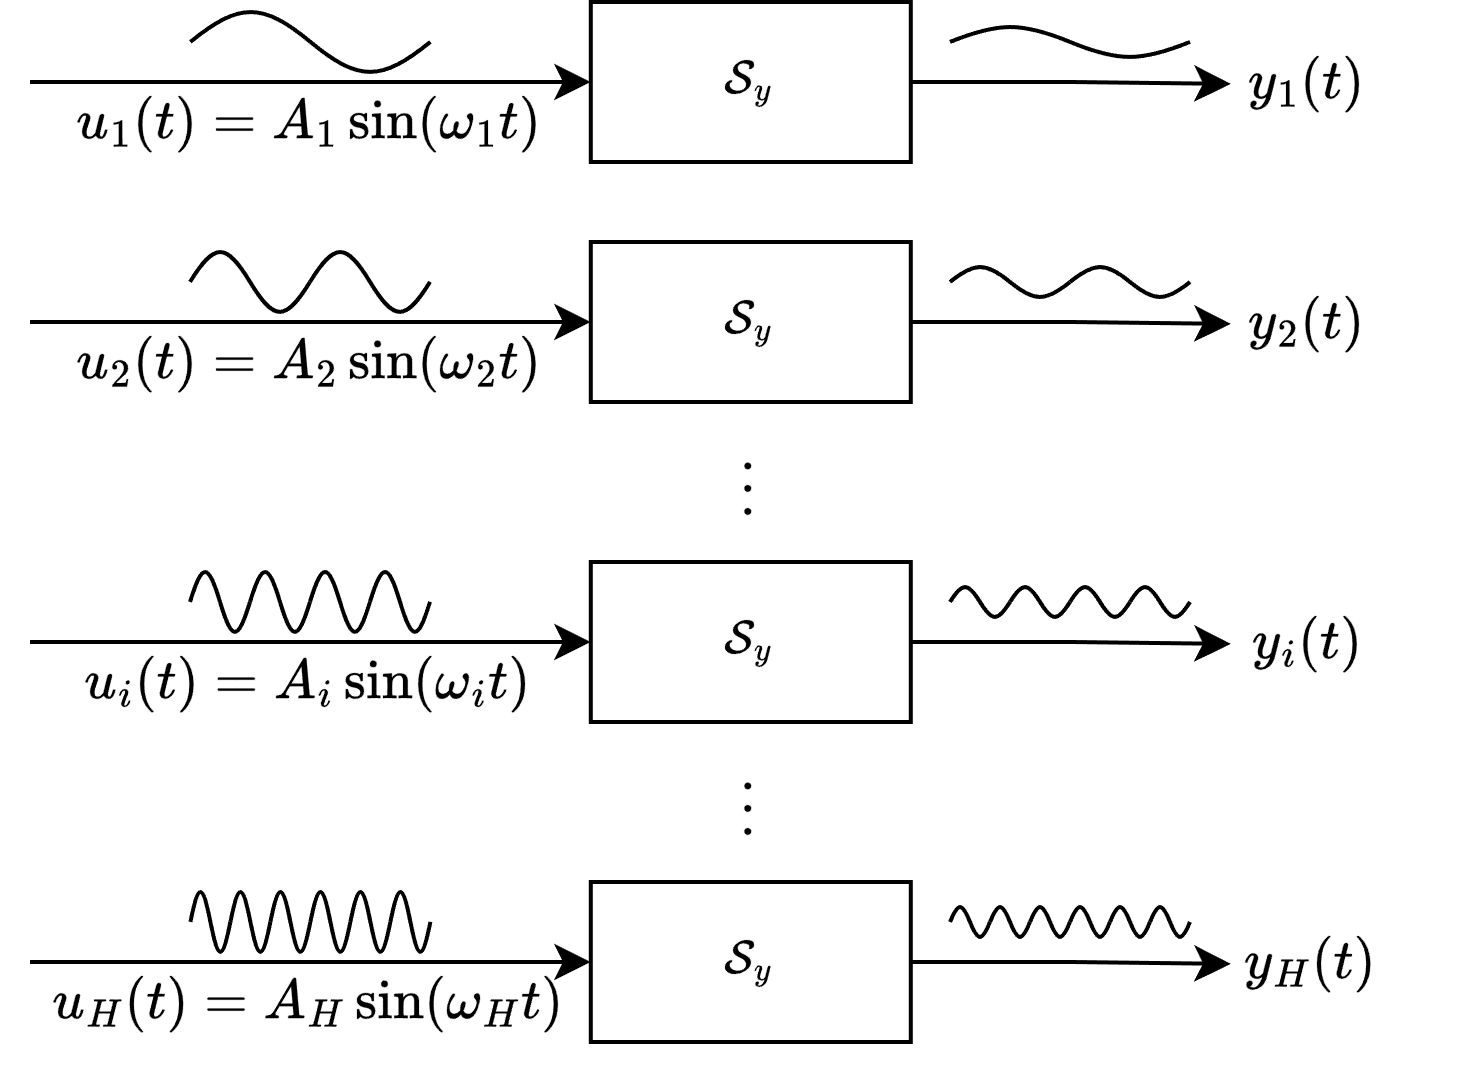
\includegraphics[width=0.6\linewidth]{images/exp.png}
\end{figure}
Upon completion of all experiments, we obtain $H$ independent datasets. 
The $i$-th dataset comprises input-output pairs:
\[\left\{u_i(1),u_i(2),\dots, u_i(N)\right\} \quad \left\{y_i(1),y_i(2),\dots, y_i(N)\right\}\]

\paragraph*{Choice of the amplitudes}
While the amplitudes of the sinusoidal inputs can be uniform across experiments, it's common practice for them to decrease gradually. 
This adjustment ensures that the amplitudes align with the system's actuation limits, thus providing a more realistic representation of operating conditions.

\subsection{Data gathering}
Let's delve into the specifics of the $i$-th experiment. 
\begin{figure}[H]
    \centering
    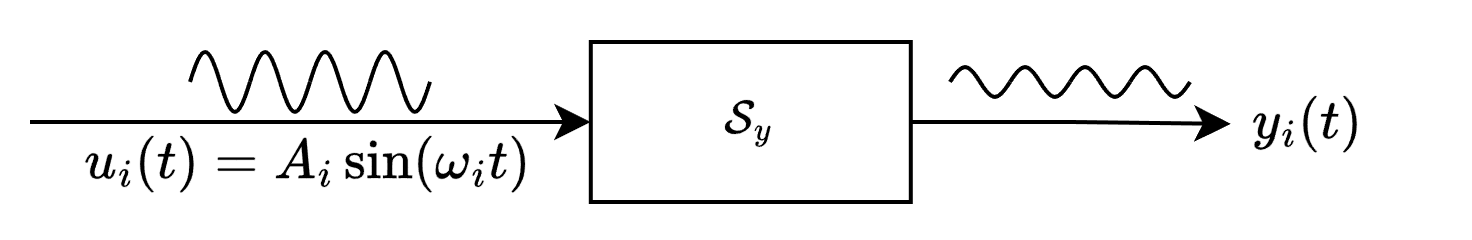
\includegraphics[width=0.6\linewidth]{images/exp1.png}
\end{figure}
For our analysis, we operate under the assumption that the system is linear and time-invariant. 
This assumption allows us to employ the theorem of frequency response for linear time-invariant systems
\begin{theorem}[Frequency response for linear time invarinat systems]
    If the input is a sinusoid of frequency $\omega_i$, the output must also be a sinusoid of frequency $\omega_i$, albeit with potentially different amplitude and phase.
\end{theorem}
However, in real-world scenarios, the output $y_i(t)$ deviates from a perfect sinusoid due to various non-ideal factors:
\begin{itemize}
    \item Measurement noise affecting the output.
    \item Internal noises within the system.
    \item Small non-linear effects, which can often be considered negligible.
\end{itemize}
Note that we are looking for a linear approximation of the system even if the system is slightly nonlinear. 
Let's call $\hat{y}_i(t)$ the perfect ideal sinusoid approximation of $f_i(t)$, that is the result of the experiment without the noise. 
We are trying to solve a classical modelling problem where our model for $y_i(t)$ is:
\[\hat{y}_i(t)=B_i\sin\left(\omega_i t+\varphi_i\right)\]
Or: 
\[\hat{y}_i(t)=a_i\sin\left(\omega_i t\right)+b_i\cos\left(\omega_i t\right)\]
They are equivalent models of a sinusoid, both with two parameters to be estimated. 

\paragraph*{Identification of parameters with amplitude-amplitude model}
We opt for the second model due to its linearity with respect to the parameters, facilitating parameter estimation.
We estimate $\hat{a}_i$ and $\hat{b}_i$ by treating it as a classical supervised parametric identification problem, with the following performance index:
\[J_N(a_i,b_i)=\dfrac{1}{N}\sum_{t=1}^N\left(y_i(t)-\left(a_i\sin(\omega_it)+b_i\cos(\omega_it)\right)\right)^2\]
This index represents the sample variance of the modeling error. 
The parameters are then obtained by minimizing this index:
\[\left\{\hat{a}_i,\hat{b}_i\right\}=\argmin_{a_i,b_i}J_N(a_i,b_i)\]
Since the model is linear with respect to the parameters, $J_N(a_i,b_i)$ is also linear. 
We can therefore minimize the performance index by solving the following system of equations:
\[\begin{bmatrix} \sum_{i}^N \sin^2(\omega_it) & \sum_{i}^N \sin(\omega_it)\cos(\omega_it) \\ \sum_{i}^N \sin(\omega_it)\cos(\omega_it) & \sum_{i}^N \cos^2(\omega_it) \end{bmatrix}\cdot\begin{bmatrix} a_i \\ b_i \end{bmatrix}=\begin{bmatrix} \sum_{i}^N y_i(t)\sin(\omega_it) \\ \sum_{i}^N y_i(t)\cos(\omega_it) \end{bmatrix}\]
Thus, the solution becomes:
\[\begin{bmatrix} \hat{a}_i \\ \hat{b}_i \end{bmatrix}=\begin{bmatrix} \sum_{i}^N \sin^2(\omega_it) & \sum_{i}^N \sin(\omega_it)\cos(\omega_it) \\ \sum_{i}^N \sin(\omega_it)\cos(\omega_it) & \sum_{i}^N \cos^2(\omega_it) \end{bmatrix}^{-1}\cdot\begin{bmatrix} \sum_{i}^N y_i(t)\sin(\omega_it) \\ \sum_{i}^N y_i(t)\cos(\omega_it) \end{bmatrix}\]
This represents the Least Squares solution to the identification problem.

\paragraph*{Identification of parameters with amplitude-phase model}
We consider the expression for $\hat{y}_i(t)$ in the amplitude-phase model:
\[\hat{y}_i(t)=\hat{B}_i\sin\left(\omega_i t+\hat{\varphi}_i\right)=\hat{B}_i\sin(\omega_i)\cos(\hat{\varphi}_i)+\hat{B}_i\cos(\omega_i)\sin(\hat{\varphi}_i)\]
Matching this expression to the amplitude-amplitude model, we find:
\[\begin{cases} \hat{B}_i\cos(\hat{\varphi}_i)=\hat{a}_i \\ \hat{B}_i\sin(\hat{\varphi}_i)=\hat{b}_i \end{cases}\]
This leads to:
\[\dfrac{\hat{a}_i}{\hat{b}_i}=\dfrac{\cos(\hat{\varphi}_i)}{\sin(\hat{\varphi}_i)}\rightarrow \hat{\varphi}_i=\arctan\left(\dfrac{\hat{b}_i}{\hat{a}_i}\right)\]
And we can also obtain $\hat{B}_i$ as:
\[\hat{B}_i=\dfrac{\frac{\hat{a}_i}{\cos(\hat{\varphi}_i)}+\frac{\hat{b}_i}{\sin(\hat{\varphi}_i)}}{2}\]
Thus, the two representations are equivalent.

In the end, we have:
\[y_i(t)\approx \hat{y}_i(t)=\hat{B}_i\sin(\omega_it+\hat{\varphi}_i)\]
This cleaning procedure is repeated for all $H$ signals.
After completing this process, we acquire $H$ complex numbers:
\[\left\{\hat{B}_i,\hat{\varphi}_i\right\}\rightarrow\dfrac{\hat{B}_i}{A_i}e^{j\hat{\varphi}_i}\]

We have $H$ complex numbers, each representing an estimated value of the frequency response of the system.
According to the frequency response theorem, if the input is $A_i\sin(\omega_it)$, then the output is $\hat{B}_i\sin\left(\omega_it+\hat{\varphi}\right)$. 

These $H$ numbers can be plotted in amplitude and phase. 
\begin{figure}[H]
    \centering
    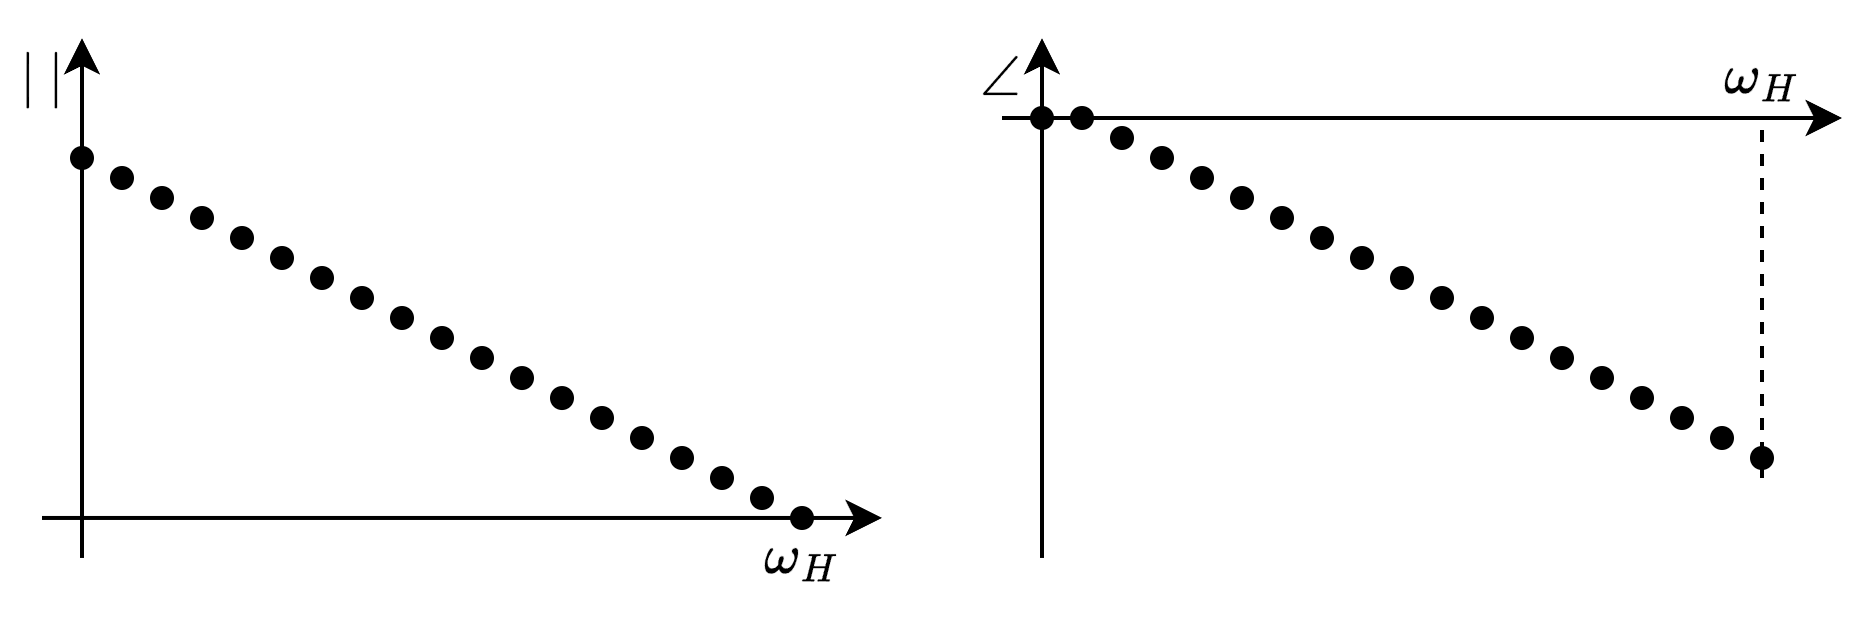
\includegraphics[width=0.6\linewidth]{images/amp.png}
    \caption{Amplitude and phase of samples $H$}
\end{figure}

\subsection{Remarks}
\paragraph*{Selection of the maximum explored bandwidth}
Determining a meaningful bandwidth for the control system is crucial. 
Often, we are provided with the bandwidth of the control system, denoted as $\omega_C$. 
A prudent selection for the maximum explored bandwidth would be:
\[\omega_H\approx 3 \times \omega_C\]
This choice ensures that the explored bandwidth sufficiently covers the relevant frequency range for the control system, enabling comprehensive analysis and effective model development.

\paragraph*{Precision}
In certain cases, achieving higher precision in the model, particularly in specific frequency ranges such as around resonances, becomes essential. 
\begin{figure}[H]
    \centering
    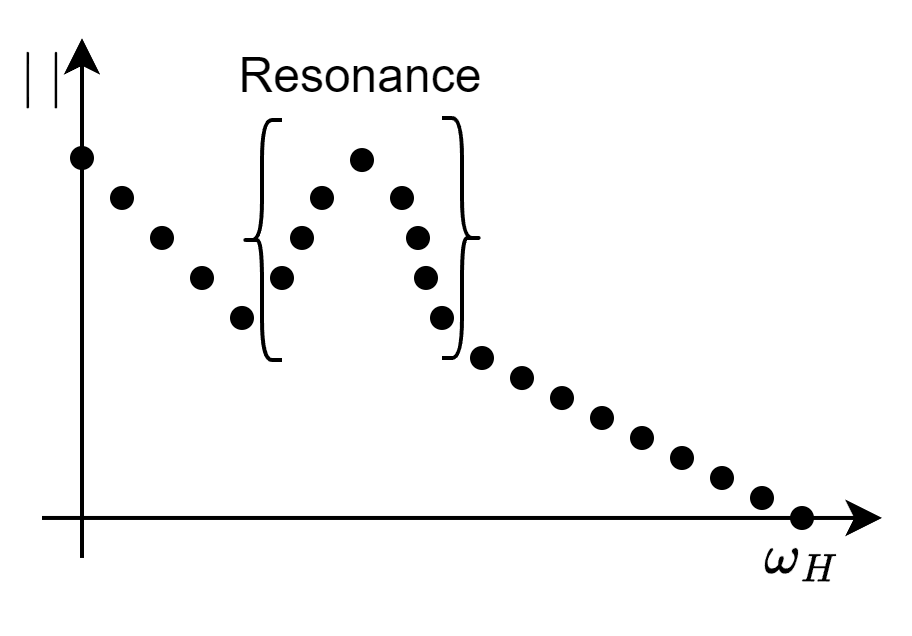
\includegraphics[width=0.4\linewidth]{images/res.png}
    \caption{Resonance}
\end{figure}
Here, our aim is to concentrate on the region with the resonance for greater accuracy.

To address this requirement, we employ non-uniform weights. Within the critical zone, frequencies $\omega_i$ carry more weight than those outside this area. 
Consequently, the performance index takes the form:
\[\tilde{J}_N(\boldsymbol{\theta})=\dfrac{1}{H}\sum_{i=1}^{H}\gamma_i\left(\left\lvert W(e^{j\omega_i},\boldsymbol{\theta})-\dfrac{\hat{B}_i}{A_i}e^{j\hat{\varphi}_i} \right\rvert^2 \right)\]
Here, $\gamma_i$ denotes the weight assigned to the frequency $\omega_i$.

Alternatively, a similar effect can be achieved by oversampling the critical frequency range.
\begin{figure}[H]
    \centering
    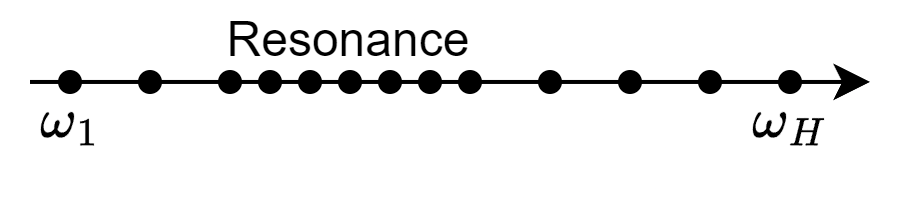
\includegraphics[width=0.5\linewidth]{images/res1.png}
    \caption{Oversampling}
\end{figure}
By conducting numerous experiments in the critical region, we obtain a non-uniformly spaced distribution, thereby enhancing precision where it is most needed.

\paragraph*{Single experiment}
In some cases, instead of conducting multiple individual sinusoidal experiments, a single, extended experiment is performed wherein $u(t)$ is a sinusoidal sweep. 
This results in a slowly time-varying frequency sinusoidal signal that spans from $\omega_1$ to $\omega_H$.
The performance index is computed as:
\[J(\boldsymbol{\theta})=\dfrac{1}{N}\sum_{i=1}^{N}\left(\left\lvert \hat{W}(e^{j\omega_i})-W(e^{j\omega_i},\boldsymbol{\theta})\right\rvert^2\right)\]
This index quantifies the deviation between the measured frequency response $\hat{W}(e^{j\omega_i})$ and the model-based response $W(e^{j\omega_i},\boldsymbol{\theta})$ across the range of frequencies considered.